\documentclass[10pt, table, dvipsnames,xcdraw,handout]{beamer}
\usetheme[progressbar=frametitle]{metropolis}
\usepackage{appendixnumberbeamer}
\usetikzlibrary{arrows.meta, positioning, quotes}
\usepackage[shortlabels]{enumitem}
\usepackage{xcolor}
\usepackage{mathtools}
\usepackage{dsfont}

\usepackage{caption}


\usepackage{cancel}

\newcommand\hcancel[2][black]{\setbox0=\hbox{$#2$}%
\rlap{\raisebox{.45\ht0}{\textcolor{#1}{\rule{\wd0}{1pt}}}}#2} 


\usepackage{booktabs}
\usepackage[scale=2]{ccicons}

\usepackage{pgfplots}
\usepgfplotslibrary{dateplot}

\usepackage{xspace}
\newcommand{\themename}{\textbf{\textsc{metropolis}}\xspace}
\newcommand{\cb}{\cellcolor{blue!25}}


% Notation:
\newcommand{\cT}{\ensuremath{\mathcal{T}}}
\newcommand{\cD}{\ensuremath{\mathcal{D}}}
\newcommand{\cX}{\ensuremath{\mathcal{X}}}
\newcommand{\cY}{\ensuremath{\mathcal{Y}}}
\newcommand{\cZ}{\ensuremath{\mathcal{Z}}}
\newcommand{\cH}{\ensuremath{\mathcal{H}}}
\newcommand{\cG}{\ensuremath{\mathcal{G}}}

\newcommand{\bR}{\ensuremath{\mathbb{R}}}
\newcommand{\bN}{\ensuremath{\mathbb{N}}}
\newcommand{\bP}{\ensuremath{\mathbb{P}}}
\newcommand{\bT}{\ensuremath{\mathbb{T}}}
\newcommand{\bL}{\ensuremath{\mathbb{L}}}

\newcommand{\bfX}{\ensuremath{\mathbf{X}}}
\newcommand{\bfY}{\ensuremath{\mathbf{Y}}}
\newcommand{\bfy}{\ensuremath{\mathbf{y}}}
\newcommand{\bfD}{\ensuremath{\mathbf{D}}}

\def\layersep{2.5cm}

% Tikz seys
\tikzset{cross/.style={cross out, draw, 
         minimum size=2*(#1-\pgflinewidth), 
         inner sep=0pt, outer sep=0pt}}

\title{Machine Learning I}
\subtitle{Lecture 16: Cluster Analysis Part III}
% \date{\today}
\date{}
\author{Nathaniel Bade}
\institute{Northeastern University Department of Mathematics}
% \titlegraphic{\hfill\includegraphics[height=1.5cm]{logo.pdf}}

\begin{document}

\maketitle

\begin{frame}{Table of contents}
  \setbeamertemplate{section in toc}[sections numbered]
  \tableofcontents[hideallsubsections]
\end{frame}


%%%%%%%%%%%%%% Slidshow Start %%%%%%%%%%%%%% 


%Notes: 4 kinds of clusering: Centroid based/kmeans, connecctivity based, density based, distribution based. 
%
% What metrics can we use to evalaute scattering? (internal) Scatter crieteria, silloett coeffcient, (external) mutial information, 
% 
%
% Association rules and merket basket analysis. 
%
%
%
%



\section{Spectral Clustering}
\begin{frame}[fragile]{Spectral Clustering}
  \begin{minipage}[t][0.5\textheight][t]{\textwidth}
	\centering \includegraphics[height=0.5\textheight]{L15Spetral.png} 
  \end{minipage}
  \vfill
\begin{minipage}[t][0.5\textheight][t]{\textwidth}
Spectral clustering uses graph theory methods to detect strings of locally close points. Much like DBSCAN and single-linkage hierarchical clustering, spectral clustering is an algorithm that finds clusters by considering only local neighborhoods around a point. \pause Unlike those method however, it is somewhat more statistically stable under resampling.
\end{minipage}
\end{frame}



\begin{frame}[fragile]{Similarity Graphs}
  \begin{minipage}[t][0.5\textheight][t]{\textwidth}
	\centering \includegraphics[height=0.5\textheight]{L17Adj.png}\includegraphics[height=0.4\textheight]{L17Sample_graph.png} 
  \end{minipage}
  \vfill
\begin{minipage}[t][0.5\textheight][t]{\textwidth}
The starting point is an $N\times N$ matrix of pairwise \textbf{similarities} or \textbf{weights} $W_{ii'} \geq 0$ between observed points. This matrix allows us to form the \textbf{similarity graph}.\pause 

The similarity graph may be dense if all weights are included, or sparse if not all connections are included. 
\end{minipage}
\end{frame}



\begin{frame}[fragile]{Similarity Graphs}
  \begin{minipage}[t][0.5\textheight][t]{\textwidth}
	\centering \includegraphics[height=0.5\textheight]{L17Adj.png}\includegraphics[height=0.4\textheight]{L17Sample_graph2.png} 
  \end{minipage}
  \vfill
\begin{minipage}[t][0.5\textheight][t]{\textwidth}
There are three standard (roughly equivalent) ways to think forming clusters from a similarity graph: 
\begin{itemize}
\item[] Graph partitioning by cutting lowest weight connections. 
\end{itemize}
\end{minipage}
\end{frame}


\begin{frame}[fragile]{Similarity Graphs}
  \begin{minipage}[t][0.5\textheight][t]{\textwidth}
	\centering \includegraphics[height=0.5\textheight]{L17Adj.png}\includegraphics[height=0.4\textheight]{L17Sample_graph3.png} 
  \end{minipage}
  \vfill
\begin{minipage}[t][0.5\textheight][t]{\textwidth}
There are three standard (roughly equivalent) ways to think forming clusters from a similarity graph: 
\begin{itemize}
\item[] Graph partitioning by cutting lowest weight connections. 
\item[] Random walk with transition threshold $T$.
\end{itemize}
\end{minipage}
\end{frame}

\begin{frame}[fragile]{Similarity Graphs}
  \begin{minipage}[t][0.5\textheight][t]{\textwidth}
	\centering \includegraphics[height=0.5\textheight]{L17Adj.png}\includegraphics[height=0.4\textheight]{L17Sample_graph4.png} 
  \end{minipage}
  \vfill
\begin{minipage}[t][0.5\textheight][t]{\textwidth}
There are three standard (roughly equivalent) ways to think forming clusters from a similarity graph: 
\begin{itemize}
\item[] Graph partitioning by cutting lowest weight connections. 
\item[] Random walk with transition threshold $T$.
\item[] Perturbing away from the case of an ideal separation where 0 wights separate true connected clusters.  
\end{itemize}
\end{minipage}
\end{frame}


\begin{frame}[fragile]{Sparse Graphs}
In addition, there are three ways to ``sparsify'' the graph if we want to trim some weights:\pause
\begin{itemize}
\item[] $K$-neighbors: Only the $K$ closest points $x_{i'}$ to each point $x_i$ are included in the graph. Edges are weighted by $W_{ii'}$ as before.  \pause
\item[] $K$-mutual neighbors: A weight is only nonzero if $x_{i'}$ is one of the $K$ points closest to $x_i$ and $x_{i'}$ is one of the $K$ closest points to $x_{i'}$. This enforces symmetry on the graph. Edges are weighted by $W_{ii'}$ as before. \pause
\item[] $\epsilon$-neighborhood: Weights of all points outside an $\epsilon$ ball of $x_i$ are set to 0. In this case, weights may be computed as before, but it is also common to set all nonzero weights to 1. \pause
\end{itemize}
Of course, we can also consider the fully connected graph. 
\end{frame}


\begin{frame}[fragile]{Sparse Graphs}
  \begin{minipage}[t][0.7\textheight][t]{\textwidth}
	\centering \includegraphics[height=0.7\textheight]{L17Sparse.png}
  \end{minipage}
  \vfill
\begin{minipage}[t][0.3\textheight][t]{\textwidth}
In this example, we see the difference between $K$-NN, mutual $K$-NN and neighborhood fitting. Note that the latter two can classify outliers. 
\end{minipage}
\end{frame}

\begin{frame}[fragile]{Motivating Result}
Motivating result: Let the \textbf{graph Laplacian} be the $N\times N$ matrix $L = D-W$, where $D$ is the diagonal matrix $D_{ii'} = \sum_{i'=1}^N W_{ii'}$ and $W$ is the symmetric matrix of positive weights. Then $L$ satisfies the following:

\textbf{1)} $L$ is symmetric and positive definite.

\textbf{2)} The smallest eigenvalue of $L$ is 0, and the corresponding eigenvector is $\mathbb{1}$. 

\textbf{3)} For $v\in \mathbb{R}^N$,
$$
v^TLv = \frac12 \sum_{i,i'} W_{ii'}(v_i-v_{i'})^2
$$


The first fact is obvious, the second comes from the fact that by the definition of $D_{ii'}$, each row sums of 1. The third we will prove shortly. 

\end{frame}



\begin{frame}[fragile]{Motivating Result}
\textbf{Proposition:} Let $G$ be an graph with non-negative symmetric weights. Then the multiplicity $K$ of the eigenvalue 0 of $L$ is the number of connected components of $G$. The eigenspace is spanned by the indicator vectors $\mathbf{1}_{C_1},\ldots, \mathbf{1}_{C_{K}}$.\pause


\textbf{Proof:} For $K=1$, the graph is connected. Assume $v$ is an eigenvector with eigenvalue 0. Then 
$$
0 = v^TLv = \frac12 \sum_{i,i'} W_{ii'}(v_i-v_{i'})^2\,.
$$
Since the $W_{ii'}$ are non-negative, for each $i,i'$ either $W_{ii'}$ is zero or $v_i = v_{i'}$. Therefore if two vertices are connected, $v_i = v_{i'}$. Therefore $v$ must be constant on the whole connected component. This show both that there is an eigenvector with eigenvalue 0, and that it is unique. 
\end{frame}



\begin{frame}[fragile]{Motivating Result}
Now, assume we have $K$ connected components. We can reorder the indices so that the connected components are sequential in the indices. Then, $W$ is block diagaonal, and so is $L$:
$$
L = \left(
\begin{matrix}
L_1&&&\\
&L_2&&\\
&&\ddots&\\
&&&L_K
\end{matrix}
\right)
$$\pause
Since each block is a proper graph on its own, the indicator function $\mathbb{1}_{C_k}$ is the unique eigenvector  with eigenvalue 0 for each $L_k$. Since the spectrum of a block diagonal matrix is the union of its block spectra there are exactly $K$ eigenvalues with eigenvector 0. 
\end{frame}





\begin{frame}[fragile]{Sparse Graphs}
  \begin{minipage}[t][0.6\textheight][t]{\textwidth}
	\centering \includegraphics[height=0.6\textheight]{L17Sparse.png}
  \end{minipage}
  \vfill
\begin{minipage}[t][0.4\textheight][t]{\textwidth}
This is a very strong result, but it inevitably has a problem in many application: What if the graph is connected, but either only sparsely or with very low weights, as in $K$ Nearest Neighbors above? The idea is to generalize the motivating by trying to use $L$ to make optimal separating cuts in our graph. 
\end{minipage}
\end{frame}




\begin{frame}[fragile]{Graph Cut Loss}
We will enter spectral clustering through cutting. Consider the partition $C = (C_1,\ldots, C_K)$. We would like to find a cut that minimizes
$$
\text{Cut}(C) = \sum_{i=1}^K \sum_{\substack{i\in C_k \\ i'\not\in C_k}} W_{ii'}\,.
$$\pause
There are two problem: This NP hard, and (at least for $K=2$) minimizing Cut$(C)$ often just peals off a single point into one cluster. \pause 

Instead, we will solve the normalized \textbf{Ratio cut} problem:
$$
\text{RCut}(C) = \sum_{k=1}^K  \frac{1}{|C_k|} \sum_{\substack{i\in C_k \\ i'\not\in C_k}} W_{ii'}\,.
$$
\end{frame}




\begin{frame}[fragile]{Ratiocut}
Define the \textbf{graph Laplacian} to be the $N\times N$ matrix $L = D-W$, where $D$ is the diagonal matrix $D_{ii} = \sum_{i'=1}^N W_{ii'}$. \pause 

Let 
$$
h_k  = \frac{1}{\sqrt{|C_k|}} \mathds{1}_{C_k}
$$ 
be the $N$-vector that is $ \frac{1}{\sqrt{|C_k|}} $ in the i'th position if $x_i\in C_k$ and $0$ otherwise. \pause Let $\mathbf{H}$ be the matrix whose columns are $h_i$. \pause

\textbf{Lemma.} Ratiocut can be written
$$
\text{RCut}(C)  = \text{Tr}(\mathbf{H}^TL\mathbf{H})\,.
$$
\end{frame}



\begin{frame}[fragile]{Graph Laplacian Example}
\begin{table}[]
\small
\begin{tabular}{cc}
Graph&Laplacian matrix
\\
\includegraphics[height=0.2\textheight]{L17Graph.png} 
&
$
\left(\begin{array}{rrrrrr}
   2 & -1 &  0 &  0 & -1 &  0\\
  -1 &  3 & -1 &  0 & -1 &  0\\
   0 & -1 &  2 & -1 &  0 &  0\\
   0 &  0 & -1 &  3 & -1 & -1\\
  -1 & -1 &  0 & -1 &  3 &  0\\
   0 &  0 &  0 & -1 &  0 &  1\\
\end{array}\right)
$
\end{tabular}
\end{table}
\begin{table}[]
\small
\begin{tabular}{cc}
Degree matrix & Adjacency matrix
\\
$
\left(
\begin{array}{rrrrrr}
  2 &  0 &  0 &  0 &  0 &  0\\
  0 &  3 &  0 &  0 &  0 &  0\\
  0 &  0 &  2 &  0 &  0 &  0\\
  0 &  0 &  0 &  3 &  0 &  0\\
  0 &  0 &  0 &  0 &  3 &  0\\
  0 &  0 &  0 &  0 &  0 &  1\\
\end{array}\right)
$
&
$
\left(\begin{array}{rrrrrr}
  0 &  1 &  0 &  0 &  1 &  0\\
  1 &  0 &  1 &  0 &  1 &  0\\
  0 &  1 &  0 &  1 &  0 &  0\\
  0 &  0 &  1 &  0 &  1 &  1\\
  1 &  1 &  0 &  1 &  0 &  0\\
  0 &  0 &  0 &  1 &  0 &  0\\
\end{array}\right)
$
\end{tabular}
\end{table}
\end{frame}




\begin{frame}[fragile]{Ratiocut as an Eigenvalue Problem}
\textbf{Lemma.} Ratiocut can be written
$$
\text{RCut}(C)  = \text{Tr}(\mathbf{H}^TL\mathbf{H})\,.
$$
\textbf{Proof:} \pause For any vector $v$, 
\begin{align*}
\action<+->{
v^T L v = v^T(D-W)v &= \frac12\sum_{i}D_{ii}v^2_i - \sum_{i,i'}W_{ii'}v_iv_{i'} +   \frac12\sum_{i'}D_{i'i'}v^2_{i'}
}
\\
\action<+->{
&= \frac12 \sum_{i,i'} W_{ii'}(v_i^2-2v_iv_{i'} + v_{i'}^2)\,,
}
\\
\action<+->{
&= \frac12 \sum_{i,i'} W_{ii'}(v_i-v_{i'})^2\,.
}
\end{align*}
\action<+->{Recall in the above that $D_{ii} = \sum_{i'=1}^N W_{ii'}$.}
\end{frame}



\begin{frame}[fragile]{Ratiocut as an Eigenvalue Problem}
Applying 
\begin{align*}
v^T L v = \frac12 \sum_{i,i'} W_{ii'}(v_i-v_{i'})^2\,,
\end{align*}
to $h_k$ and noting that $(h_{ki} - h_{ki'})^2$ is only nonzero if $i\in C_k$ and $i'\not\in C_k$ we have
$$
h_k^T L h_k = \frac{1}{|C_k|} \sum_{\substack{i\in C_k \\ i'\not\in C_k}} W_{ii'}\,.
$$ \pause
Since 
$$
\text{Tr}(\mathbf{H}^TL\mathbf{H}) = \sum_{k=1}^K h_k^T L h_k \pause = 
\sum_{k=1}^K \frac{1}{|C_k|} \sum_{\substack{i\in C_k \\ i'\not\in C_k}} W_{ii'}\,,
$$\pause
we have shown 
$$
\text{RCut}(C)  = \text{Tr}(\mathbf{H}^TL\mathbf{H})\,.
$$
\hfill $\Box$
\end{frame}


\begin{frame}[fragile]{Eigenvalues of Laplacian}
Now, since 
$$
\text{RCut}(C)  = \text{Tr}(\mathbf{H}^TL\mathbf{H})\,,
$$
we know how to minimize $\text{RCut}(C)$: the solutions that extremize $h_k^T L h_k$ are the eigenvectors. \pause Therefore, $\text{Tr}(\mathbf{H}^TL\mathbf{H})$ will be minimized by a matrix of the smallest eigenvectors of $L$, just as for PCA \pause

The eigenvectors will not in general be of the form $h_k$ for some clustering $k$. We can see that
$$
h_k^T L h_k = \frac12 \sum_{i,i'} W_{ii'}(h_{ki}-h_{ki'})^2\,,
$$
will be minimized when $h_k$ is picked to map points with high adjacency near to eachother in the reduced space. \pause Clustering there yields a fundamentally new clustering. 
\end{frame}



\begin{frame}[fragile]{Eigenvalues of Laplacian}
  \begin{minipage}[t][0.7\textheight][t]{\textwidth}
	\centering \includegraphics[height=0.7\textheight]{L17SpectralComp.png} 
  \end{minipage}
  \vfill
\begin{minipage}[t][0.3\textheight][t]{\textwidth}
Here, we see the projection onto the first nontrivial eigenvectors of $L$, as well the eigenvalues plotted against eachother. 
\end{minipage}
\end{frame}






\begin{frame}[fragile]{Example: PCA vs Spectral Projection}
  \begin{minipage}[t][0.7\textheight][t]{\textwidth}
	\centering \includegraphics[width=0.45\textwidth]{L17PCA.png}\includegraphics[width=0.45\textwidth]{L17SpectralClust.png} 
  \end{minipage}
  \vfill
\begin{minipage}[t][0.3\textheight][t]{\textwidth}
We compare the principle component projection from the MNIST dataset to the spectral projection. We see a similar structure between the two, although one set is not convex while the other is. 
\end{minipage}
\end{frame}



\begin{frame}[fragile]{Summary}
We should mention the advantages and disadvantages of spectral clustering:\pause
\begin{itemize}
\item[] Works well on hard, nonconvex problems. \pause
\item[] Obtain low dimensional representations as part of process. \pause
\item[] Empirically very successful. \pause
\item[] Flexibly definable for a wide variety of dissimilarity measures. 
\end{itemize}
\end{frame}


\begin{frame}[fragile]{Summary}
We should mention the disadvantages of spectral clustering:\pause
\begin{itemize}
\item[] We must choose $K$. \pause
\item[] We must choose a similarity measure, and Gaussian similarity may not be the best. \pause
\item[] Can be very computationally expensive on large datasets. \pause
\item[] Low dimensional feature space doesn't have an intuitive meaning.
\end{itemize}
\end{frame}


\begin{frame}[fragile]{Spectral Clustering}
Review Questions:

How does the dissimilarity come into spectral clustering? What would be the effect of changing from a dissimilarity define by the euclidean norm and the $\ell_1$ norm?

Spectral clustering involves finding the eigenvalues of an $N\times N$ matrix. For a general matrix this may be very hard, but for a sparse matrix there are good methods. What are the pros and con of using the different sparsifying methods discussed here?

What are the columns of the matrix $\mathbf{H}$ representing? What form do we expect the columns to take after we find the eigenvectors of $L$? Do we see them taking that form in slide 43? Hint: Think about how we defined $h_k$. 

\end{frame}



\section{Probabilistic Cluster Analysis: Gaussian Mixtures}


\begin{frame}[fragile]{Probabilistic Cluster Analysis}
  \begin{minipage}[t][0.5\textheight][t]{\textwidth}
	\centering \includegraphics[height=0.5\textheight]{L17MultEx.png}
  \end{minipage}
  \vfill
\begin{minipage}[t][0.5\textheight][t]{\textwidth}
Many times clusters fundamentally overlap, with individual data points not clearly belonging to one cluster or the other even though distinct clusters still clearly exist. \pause Even in high dimensional datasets we might not expect our features to completely separate the data. 
\end{minipage}
\end{frame}


\begin{frame}[fragile]{Mixture Models}
  \begin{minipage}[t][0.5\textheight][t]{\textwidth}
	\centering \includegraphics[height=0.5\textheight]{L17MultEx1.png}
  \end{minipage}
  \vfill
\begin{minipage}[t][0.5\textheight][t]{\textwidth}
In such cases we should allow ourselves to fit \textbf{mixture models} to the data. Mixture models are a form of additive modeling, and we are constrained as usual by the complexity of the constructed features of our assumed distributions. 
\end{minipage}
\end{frame}


\begin{frame}[fragile]{Mixture Models}
  \begin{minipage}[t][0.5\textheight][t]{\textwidth}
	\centering \includegraphics[height=0.5\textheight]{L17MultEx2.png}
  \end{minipage}
  \vfill
\begin{minipage}[t][0.5\textheight][t]{\textwidth}
In a \textbf{Gaussian mixture model} we try to fit Gaussian distributions to $K$ clusters. That is, we assume each label is distributed as a Gaussian:
$$
p(x_i | y_i = k) \sim \mathcal{N}(\mu_k,\Sigma_k) \,.
$$\pause 
The probability a point $x_i$ belongs to cluster $k$ is then $p_{ik} = p(z_i = k | x_i)$, where
$
\sum_{k=1}^K p_{ik} = 1\,.
$
\end{minipage}
\end{frame}



\begin{frame}[fragile]{Mixture Models and Expectation Maximization}
Formally, would like to find a probability function
$$
p(x | \theta) = \sum_{k=1}^K \phi_k \mathcal{N}(x | \mu_k,\Sigma_k)\,,
$$\pause
where $\mu_k$ denotes the Gaussians mean, and $\Sigma_k$ denotes it's covariance matrix: 
$$
\mathcal{N}(x | \mu,\Sigma) = \frac{1}{\sqrt{(2\pi)^K|\Sigma|}}\exp\left(-\frac12(x-\mu)^T\Sigma^{-1}(x-\mu)\right)\,.
$$  \pause
The $\theta = \{\mu_k,\Sigma_k,\phi_k\}$ collect all parameters, and $\sum \phi_k = 1$. 
\end{frame}



\begin{frame}[fragile]{Mixture Models and Expectation Maximization}
Given a data set $\cT$, we want to maximize the likelihood that $\cT$ was drawn (i.i.d.) from $p(x | \theta)$. \pause The likelihood of getting the data we observe is
$$
\textbf{Likelihood:}\hspace{2em}L(\cT, \theta) = \prod_{i=1}^N p(x_i|\theta)\,.\hspace{6em}
$$\pause
Our goal then is to find $\theta$ that maximize $L(\cT, \theta)$. The \textbf{expectation maximization} algorithm is a popular tool for solving MLE problems. The EM algorithm attempts to maximize the log likliehood
$$
\ell(\cT, \theta) = \log L(\cT, \theta)  =  \sum_{i=1}^N \log p(x_i|\theta)\,.
$$\pause
Unlike for linear methods, direct maximization in this case involves derivatives of a log of a sum which are hard to find an analytic solution for.
\end{frame}



\begin{frame}[fragile]{Mixture Models and Expectation Maximization}
 Expectation Maximization uses an iterative method that lowers the loss at each step. The algorithm proceeds in two steps:
\begin{itemize}
\item[] \textbf{Expectation Step:} For a set of parameters $\theta^{(i)}$, calculate exceptions $p_{ik}$ of the component assignment for each datapoint $x_i$.\pause 
\item[] \textbf{Maximization Step:} Then, maximize the expectations calculated the previous step with respect to the model parameters. \pause
\end{itemize}
Lets run through it.
\end{frame}


\begin{frame}[fragile]{Mixture Models and Expectation Maximization}
\textbf{Initialization:} Randomly assign training samples to clusters $C_k$, set $\mu_k$, $\Sigma_k$ to the in cluster sample mean and variance respectively, and set $\phi=\frac1K$. \pause

\textbf{Expectation Step:} Calculate the probability $x_i$ is generated by component $C_k$:
$$
p_{ik} = \frac{\phi_k \mathcal{N}(x_i | \mu_k,\Sigma_k) }{\sum_{j=1}^K \phi_j \mathcal{N}(x | \mu_j,\Sigma_j)}\,.
$$


\end{frame}





\begin{frame}[fragile]{Mixture Models and Expectation Maximization}
\textbf{Maximization Step:} Using $p_{ik}$ we can calculate the parameters that would maximize the expectation as follows: The number per cluster is approximately
$$
\hat{N}_k = \sum_{i=1}^N p_{ik}\,,\hspace{2em}\text{so}\hspace{2em} \hat \phi = \frac{\hat N_k}{N}\,.
$$\pause
The mean can be computed as the weighted centroid
$$
\hat\mu_k = \frac{1}{\hat N_k}\sum_{i=1}^N p_{ik}x_i\,,
$$\pause
and the variance is the weighted covariance
$$
\hat\Sigma_k = \frac{1}{\hat N_k}\sum_{i=1}^N p_{ik}(x_i-\hat \mu _k)(x_i-\hat \mu _k)^T\,.
$$
\end{frame}





\begin{frame}[fragile]{Mixture Models}
  \begin{minipage}[t][0.5\textheight][t]{\textwidth}
	\centering \includegraphics[height=0.5\textheight]{L17Guassian.png}
  \end{minipage}
  \vfill
\begin{minipage}[t][0.5\textheight][t]{\textwidth}
Compare the actual labeling on the left with the Guassian labeling on the right. While all the points along the strip are classified as being a part of Cluster 1 this is probably just because Cluster 1 has lower variance, in fact the probabilities are around .5 along the intersecting strip. 
\end{minipage}
\end{frame}





\begin{frame}[fragile]{Mixture Models}
  \begin{minipage}[t][0.7\textheight][t]{\textwidth}
	\centering \includegraphics[height=0.7\textheight]{L17GMM.png}
  \end{minipage}
  \vfill
\begin{minipage}[t][0.3\textheight][t]{\textwidth}
We can see several fittings of the Iris data set using differently shaped clusters. Here, the dots are the training points and the crosses are the test points. 
\end{minipage}
\end{frame}



\begin{frame}[fragile]{Mixture Model Clustering}
Review Questions:

Does mixture model clustering require knowing the labels beforehand?

Assume you have three, well separated Gaussian clusters, but you only use $K=2$ clusters for your fit. What happens? 

How would you use a Guassian Mixture Model to fit the latitude and longitude for the NYAirBnB dataset?
\end{frame}




\section{Evaluating Clustering: Internal Measures}

\begin{frame}[fragile]{Clustering Criteria}
Evaluating clustering falls into two rough categories:\pause

\textbf{Criteria internal to a dataset:}
Scattering Criteria: Minimize the intracluster variance and maximize the intercluster variance. Internal criteria are relative measures of clustering, and should always be understood not as absolute evaluations but as a way of ranking many potential clustering against eachother. 

\textbf{External criteria:}
The comparison of clusters to a true labeling or to a strong underlying ground truth. This may be precision/recall, the probability of randomly guessing a labeling, or the deviation from an assumed model. 
\end{frame}





\begin{frame}[fragile]{Internal Measures: Scattering Criteria}
The total cluster variance can be decomposed into the inter-(between)-scatter variance and the intra-(within)-scatter variance
$$
\text{Cov} = \sum_{i=1}^N (x_i-\mu)(x_i-\mu)^T = S_W+ S_B \,,
$$\pause
where
\begin{flalign*}
\text{Total Intra}&&S_W = \sum_{j=1}^K  \sum_{x\in C_j}(x - \mu_j)(x - \mu_j)^T\,,&&
\\
\text{Total Inter}&&S_B = \sum_{j=1}^K |C_j| (\mu_j - \mu)(\mu_j - \mu)^T\,. &&
\end{flalign*}

\end{frame}







\begin{frame}[fragile]{Internal Measures: Calinski-Harabasz Index}
The Calinski-Harabaz (CH) index is defined as
$$
CH = \frac{\text{Tr}(S_B)}{\text{Tr}(S_W)}\,.
$$\pause
The trace being the sum over eigenvalues, the index will be large when the between group variance is large and the within group variance is small. \pause

The Calinski-Harabasz (CH) index is a fast to compute, and larger when the clusters are dense and well separated. On the other hand, it is generally higher for convex clusters than for the large, density based clusters found by algorithms like DBSCAN.
\end{frame}





\begin{frame}[fragile]{Internal Measures: Calinski-Harabasz Index}
 \begin{minipage}[t][0.5\textheight][t]{\textwidth}
	\centering \includegraphics[height=0.5\textheight]{L15CHIndex.png} 
  \end{minipage}
  \vfill
\begin{minipage}[t][0.5\textheight][t]{\textwidth}
We can use the CH index to compare clustering methods and to compute $K$. Plotting the CH index against $K$, we look for local maxima. These indicate that adding another cluster reduces the between cluster variance, without a sufficient compensating reducing in within cluster variance. Above, we could guess that 4 or 6 clusters was the optimal number. 
\end{minipage}
\end{frame}



\begin{frame}[fragile]{Internal Measures: Calinski-Harabasz Index}
	\centering \includegraphics[width=\textwidth]{L15CHIndex2.png} 
\end{frame}






\begin{frame}[fragile]{Internal Measures: Calinski-Harabasz Index}
 \begin{minipage}[t][0.5\textheight][t]{\textwidth}
	\centering \includegraphics[height=0.5\textheight]{L15CHIndex3.png} 
  \end{minipage}
  \vfill
\begin{minipage}[t][0.5\textheight][t]{\textwidth}
It is also important to not that it is not the absolute value of the CH index that matters, but more the ruggedness of the curve. If we let the number of clusters grow to 100, the curve continues to increase, but steadily. 
\end{minipage}
\end{frame}






\begin{frame}[fragile]{Internal Measures: Silhouette Coefficient}
The silhouette coefficient measures how similar each data point is to it's own cluster (cohesion) compared to other clusters (separation). \pause Let $a_i$ be the average distance from $x_i$ to the other elements in the cluster
$$
a_i = \frac{1}{|C_k| - 1}\sum_{x_j\in C_k} D(x_i,x_j)\,,
$$\pause
and let $b_i$ be the smallest average distance of $x_i$ to all points in another cluster
$$
b_i = \min_{\ell\neq k} \frac{1}{|C_\ell|}\sum_{x_j\in C_\ell} D(x_i,x_j)\,.
$$\pause
Then the silhouette coefficient is for each $x_i$ is 
$$
s_i \frac{b_i - a_i}{\text{max}(a_i,b_i)}\,.
$$
\end{frame}








\begin{frame}[fragile]{Internal Measures: Silhouette Coefficient}
The mean silhouette coefficient is
$$
SC = \frac{1}{N}\sum_{i=1}^N \frac{b_i - a_i}{\text{max}(a_i,b_i)}\,.
$$
Ranges from -1 to +1, where a high value indicates that the object is well matched to its own cluster and poorly matched to neighboring clusters.\pause

The silhouette for each datapoint can also be measured individually. If most points have a silhouette near 1, then the clustering configuration is cohesive and separated. Otherwise, the clustering configuration may have an inappropriate number of clusters. \pause

The individual coefficient $s_i = \frac{b_i - a_i}{\text{max}(a_i,b_i)}$ is also a good test for outliers or misclassified points with zero values corresponding to outliers and negative values to misclassifications.
\end{frame}


\begin{frame}[fragile]{Internal Measures: Silhouette Coefficient}
 \begin{minipage}[t][0.5\textheight][t]{\textwidth}
	\centering \includegraphics[height=0.5\textheight]{L15SCScore.png} 
  \end{minipage}
  \vfill
\begin{minipage}[t][0.5\textheight][t]{\textwidth}
The mean silhouette coefficient can be used in a similar way as the CH Index to compute the proper $K$ value for clustering, but we can also get much more granular data. In the data sampled before I used Ward clustering. Using centroid, the fit becomes much less stable and so perhaps more realistic to high dimensional data.
\end{minipage}
\end{frame}


\begin{frame}[fragile]{Internal Measures: Calinski-Harabasz Index}
	\centering \includegraphics[width=\textwidth]{L15Centroid.png} 
\end{frame}




\begin{frame}[fragile]{Internal Measures: Silhouette Coefficient}
 \begin{minipage}[t][0.5\textheight][t]{\textwidth}
	\centering \includegraphics[height=0.5\textheight]{L15Centroid2.png} 
  \end{minipage}
  \vfill
\begin{minipage}[t][0.5\textheight][t]{\textwidth}
Now we have two peaks, and actually we know from the previous slide that the second peak is shifted by a bad fit: a single cluster containing only 1 data point. 
\end{minipage}
\end{frame}


\begin{frame}[fragile]{Internal Measures: Silhouette Coefficient}
 \begin{minipage}[t][0.5\textheight][t]{\textwidth}
	\centering \includegraphics[height=0.5\textheight]{L15Centroid3.png} 
  \end{minipage}
  \vfill
\begin{minipage}[t][0.5\textheight][t]{\textwidth}
Lets consider the by-cluster histogram of the silhouette coefficients. The red lines indicate the mean silhouette coefficient. Looking at the clusters for $K=2$, we see a large cluster with a significant number of negative values. This indicates that we need to split this cluster, as its values are closer to other clusters than the average distance to other elements within the cluster. 
\end{minipage}
\end{frame}





\begin{frame}[fragile]{Internal Measures: Silhouette Coefficient}
 \begin{minipage}[t][0.5\textheight][t]{\textwidth}
	\centering \includegraphics[width=\textwidth]{L15Centroid4.png} 
  \end{minipage}
  \vfill
\begin{minipage}[t][0.5\textheight][t]{\textwidth}
Moving up to $K = 4- 6$, we see the appearance of the bad cluster. But also, comparing $K = 4$ to the non-outlier clusters of $K=6$, we see that in general the clusters in $K=6$ have a per cluster silhouette average in line with the total silhouette average. This implies the clusters are fairly regular. 
\end{minipage}
\end{frame}


\begin{frame}[fragile]{Internal Measures: Silhouette Coefficient}
 \begin{minipage}[t][0.5\textheight][t]{\textwidth}
	\centering \includegraphics[width=\textwidth]{L15Centroid4.png} 
  \end{minipage}
  \vfill
\begin{minipage}[t][0.5\textheight][t]{\textwidth}
Cluster 4 on the other hand has a large cluster (2) with almost all of the silhouette values below the mean silhouette value. This indicates that cluster 2 has a significantly different density, spread, or variance than the other clusters. If a better clustering exists, it may be more reliable. 
\end{minipage}
\end{frame}







\begin{frame}[fragile]{Internal Measures: Calinski-Harabasz Index}
	\centering \includegraphics[width=\textwidth]{L15CHIndex2.png} 
\end{frame}

\section{Evaluating Clustering: External Measures}



\begin{frame}[fragile]{Precision and Recall}
Consider a simple binary classification where an algorithm predicts the results of a test as positive or negative. Given knowledge of the true labeling, you can form the error matrix

\begin{table}[]
\begin{tabular}{l | ll}
  & Actually True & Actually False \\  \hline
Predicted True & True Positive (TP)  & False Positive (FP) \\
Predicted False & False Negative (FN)  &  True Negative (TN) 
\end{tabular}
\end{table}
The precision is the proportion of correctly predicted positives:
$$
P = \frac{\# TP}{\text{Predicted Positive}} = \frac{\# TP}{\# TP + \# FP}\,.
$$
while the recall is the proportion of actual positive found:
$$
R = \frac{\# TP}{\text{Actual Positive}} = \frac{\# TP}{\# TP + \# FN}\,.
$$
\end{frame}


\begin{frame}[fragile]{Precision and Recall}
In clustering, the analog of the error table is 
Correct Decisions:
\begin{itemize}
\item \textbf{TP} - Placing a pair of points with the same label in the same cluster.
\item \textbf{TN} - Place a pair of points with different labels in different clusters. 
\end{itemize}
Errors:
\begin{itemize}
\item \textbf{FP} - Placing a pair of points with different label in the same cluster.
\item \textbf{FN} - Place a pair of points with the same label in different clusters. 
\end{itemize}

While precision and recall can then be analogously defined for clustering, it is also useful to use the concepts above to simply define the total error rate, or the Rand index. 
\end{frame}



\begin{frame}[fragile]{External Measures: Rand Index}
Assume now that there is a true categorical labeling that is known and let $y\in \cY$ be the classes. Let $k$ parameterize the $K$ classes picked by clustering. 

The Rand index computes the percentage of correct classifications the clustering made by the following formula: Let $a$ be the number of pairs of elements that are in the same cluster $C$ and also have the same label in $K$. Let $b$ be the number of pairs in different sets in both $C$ and $K$. Let $P$ be the number of unordered pairs in the dataset. The Rand index is

$$
RI = \frac{a+ b}{C}
$$
\end{frame}



\begin{frame}[fragile]{External Measures: Rand Index}
Assume now that there is a true categorical labeling that is known and let $y\in \cY$ be the classes. 

The Rand index computes the percentage of correct classifications the clustering made by the following formula: Let $a$ be the number of pairs of elements that are in the same cluster $C$ and also have the same label in $K$. Let $b$ be the number of pairs in different sets in both $C$ and $K$. Let $P$ be the number of unordered pairs in the dataset. The Rand index is

$$
RI = \frac{a+ b}{P}\,.
$$\pause

An almost perfect labeling will have a score close to 1, however, the Rand index doesn't guarantee that a random label assignment will get a score close to 0. It is usually adjusted to
$$
ARI = \frac{RI - E[RI]}{\text{max}(RI) - E[RI]}\,.
$$
\end{frame}





\begin{frame}[fragile]{External Measures: Rand Index}
ARI has a couple of strong advantages:

\begin{itemize}
\item First, random labels have ARI score close to 0 while perfect labeling have an ARI score close to 1. Terrible labelings (for example,  all data in one cluster and $K-1$ singleton clusters) have negative ARI score. 

\item ARI has a bounded, meaningful range from [-1,1].

\item No assumptions are made on the cluster structure or geometry. ARI works as well for DBSCAN as for Gaussian mixtures. 
\end{itemize}
\end{frame}



\begin{frame}[fragile]{External Measures: Rand Index}
\begin{table}[]
\begin{tabular}{l | lll l l | lll}
  & C1 & C2 & C3 & &  & C1 & C2 & C3 \\ 
A & 5  & 0  & 0 & & A & 4  & 0  & 1\\
B & 0  & 3  & 2 & & B & 1  & 3  & 1\\
C & 0  & 2  & 3 & & C & 0  & 1  & 4
\end{tabular}
\end{table}


Consider the two clustering above. It may be hard to tell just by looking which has classified more pairs correctly or worse. Here, the ARI makes is very clear which clustering has correctly organized more pairs of points. 
$$
\textbf{Left ARI: } 0.4399\,,\,\,\, \textbf{Right ARI: }0.2838
$$
According to the ARI measure, the right clustering is significantly worse. This is partially because the pair waiting increases quadratically in the number of correctly separated data points. 
\end{frame}






\begin{frame}[fragile]{External Measures: Mutual Information}
The \textbf{mutual information} is
$$
I(\cY,K) = \sum_{y\in \cY, k\in K} p(y,k)\log\frac{p(y,k)}{p(y)p(k)}\,,
$$\pause
where $p(y,k)$ is the total chance of a datapoint $x_i$ with true label $y$ being in cluster $k$, $p(y)$ is the proportion of data points labeled $y$, and $p(k)$ is the proportion of data points in cluster $k$. \pause 

Mutual information measures how much knowing one of these variables reduces uncertainty about the other.
High mutual information indicates a large reduction in uncertainty; low mutual information indicates a small reduction; and zero mutual information between two random variables means the variables are independent. 
\end{frame}



\begin{frame}[fragile]{External Measures: Mutual Information}
  \begin{minipage}[t][0.5\textheight][t]{\textwidth}
	\centering \includegraphics[height=.5\textheight]{L16MutuleInformation.png} 
  \end{minipage}
  \vfill
\begin{minipage}[t][0.5\textheight][t]{\textwidth}
\begin{table}[]
\begin{tabular}{l|lll|l}
$p(y,k)$   & 1    & 2    & 3    & $p(k)$ \\ \hline
setosa     & 0    & 0    & .333 & .333   \\
versicolor & .093 & .24  & 0    & .333   \\
virginica  & .327 & .007 & 0    & .333   \\ \hline
$p(y)$     & .42  & .247 & .333 &       
\end{tabular}
\end{table}
$I(\cY, K) = 0.845$ in this example, 
\end{minipage}
\end{frame}



\begin{frame}[fragile]{External Measures: Mutual Information}
Without getting too much into the details, mutual information is used here instead of correlation because it can account for categorical variables. \pause Comparing the two, 
$$
\text{Cov}(X,Y) = \sum_{x,y}[p(x,y) - p(x)p(y)]xy\,,
$$
and 
$$
I(X,Y) = \sum_{x,y}[log(p(x,y)) - log(p(x)p(y))]p(x,y)\,,
$$\pause
we see that covariance looks at how non-independence effects the product $xy$, while mutual information measure the log of the effect of nonindependence on the mutual probability distribution. \pause In some sense here, mutual information is the covariance of the distributions.  It is subtly but directly related to the $\chi^2$ statistic. 
\end{frame}





\begin{frame}[fragile]{External Measures: Others}
There are many other scores that try to capture different aspects of the clustered data. I would encourage you to look at the excellent list maintained by Scikit Learn community:

https://scikit-learn.org/stable/modules/clustering.html

I would also encourage you to consider your own methods and methodologies. It is best to evaluate a clustering using all of the methods available, as well as a careful analysis of the confusion table. 
\end{frame}






\begin{frame}[fragile]{Review: Evaluating}
Review: 

When would you use each of the measure presented in this chapter?

Do you agree with the ARI's assesment of the validity of the clusterings in Slide 80. Why or why not? Could you modify it to account for a metric that extracts different information?

Precision and recall are two of the most common metrics for binary classification, but become more difficult to extend to multiclass classification. Assume you have $K$ labels and $K$ clusters. How could you extend  precision and recall to this case?

Assume you run a $K$-means clustering and the silhouette histogram has two large blocks, both with many negative values. What might you conclude about the shape of the clusters? What algorithm should you use instead?
\end{frame}








\section{The Theoretical Problem}

\begin{frame}[fragile]{Axiomatizing Clustering}
What distinguishes a clustering algorithm from any arbitrary function from a training set to partition space? One may try to use an axiomatic approach, for example a 2003 attempt by Kleinberg:\pause

Consider a clustering function $F(D)$ from a domain $\cX$ to its partitions that depends on a dissimilarity matrix $D$. Consider the following properties:\pause

\begin{itemize}
\item[] \textbf{Scale Invariance:} For any $\alpha>0$ the following should hold: $F(D) = F(\alpha D)$\pause
\item[] \textbf{Richness:} For every finite set $\cX$ and every partition $C = \{C_1,\ldots, C_K\}$, there exists some dissimilarity function $D$ over $\cX$ such that $F(\cX, D) = C$. \pause
\item[] \textbf{Constancy:} If $D$, $D'$ are dissimilarity functions such that for every $x,y\in \cX$, (if $x,y$ belong to the \textbf{same} cluster in $F(D)$ then $D'(x,y)\leq D(x,y)$) \textbf{and} (if $x,y$ belong to \textbf{different} clusters in $F(D)$ then $D'(x,y)\geq D(x,y)$), \textbf{then} $F(D) = F(D')$.  
\end{itemize}

\end{frame}






\begin{frame}[fragile]{Axiomatizing Clustering}
Scale invariance is an obvious requirement. Richness might seem a little strange at first but it enforces the fact that the distance function should contain all of the information about the clustering, none comes from the background space itself. \pause

\textbf{Constancy:} If $D$, $D'$ are dissimilarity functions such that for $x,y\in \cX$, if $x,y$ belong to the \textbf{same} cluster in $F(D)$ then $D'(x,y)\leq D(x,y)$ \textbf{and} if $x,y$ belong to \textbf{different} clusters in $F(D)$ then $D'(x,y)\geq D(x,y)$, \textbf{then} $F(D) = F(D')$.  \pause

Consistency is the condition that enforces the definition of clustering. Similar points should be clustered together and different points should be clustered differently. If in moving from $D$ to $D'$ the points that share a cluster get \textbf{more} similar and those don't get less similar the clustering function should find the same clusters. 

\end{frame}


\begin{frame}[fragile]{Axiomatizing Clustering}
  \begin{minipage}[t][0.5\textheight][t]{\textwidth}
	\centering \includegraphics[height=0.5\textheight]{L16GammaTrans.png}
  \end{minipage}
  \vfill
\begin{minipage}[t][0.5\textheight][t]{\textwidth}
\textbf{Constancy:} If $D$, $D'$ are dissimilarity functions such that for $x,y\in \cX$, if $x,y$ belong to the \textbf{same} cluster in $F(D)$ then $D'(x,y)\leq D(x,y)$ \textbf{and} if $x,y$ belong to \textbf{different} clusters in $F(D)$ then $D'(x,y)\geq D(x,y)$, \textbf{then} $F(D) = F(D')$. 

Consistency states that the clusters $F(D)$ should be the same as for $F(D')$. 
\end{minipage}
\end{frame}





\begin{frame}[fragile]{Axiomatizing Clustering}
\textbf{Theorem} (Kleinber, 2003) There exists no function $F$ that satisfies all three properties. \pause\newline

\textbf{Proof:} Let $\cX = \{a,b,c\}$. By richness there must be a $D$ such that $F(D) = \{\{a\},\{b\},\{c\}\}$ and another $D'$ such that $F(D') \neq F(D)$. \pause

For some value of $\alpha$, $\alpha D'(x,y)\geq D(x,y)$ for all $x,y\in \cX$. By scale invariance, $F(\alpha D') = F(D')$. \pause 

Finally, since all distinct $x$ lie in their own cluster wrt $F(D)$ and $\alpha D'(x,y) \geq D(x,y)$, consistency implies that $F(\alpha D') = F(D) = F(D')$, a contradiction. $\Box$ \pause

Note, that any two of these axioms are alright, it takes all three to result in a problem. 
\end{frame}



\begin{frame}[fragile]{Hierarchical Clustering}
  \begin{minipage}[t][0.5\textheight][t]{\textwidth}
	\centering \includegraphics[height=0.5\textheight]{L16Linkage4.png}\includegraphics[height=0.5\textheight]{L16Linkage3.png}
  \end{minipage}
  \vfill
\begin{minipage}[t][0.5\textheight][t]{\textwidth}
Relaxing each of these conditions gives new information about clustering. Lets consider how single linkage clustering interacts with these conditions. In single linkage clustering we must pick a stopping condition, that is a cutoff. 
\end{minipage}
\end{frame}


\begin{frame}[fragile]{Hierarchical Clustering}
Consider the three stopping conditions:
\begin{itemize}
\item\textbf{K-Clusters:} Stop when $K$ clusters have formed.\pause

\item\textbf{Distance Stopping:} Only combine clusters edges of dissimilarity at most $r$. \pause

\item\textbf{Scale Stopping:} Let $\alpha\in [0,1]$ and let $D_* = \text{max}(D_{ii'})$. Only combine clusters of dissimilarity at most $\alpha$. 

\end{itemize}
\textbf{Question:} Each of these conditions violates exactly one of the properties of optimal clustering. Which stopping condition violates which property?\pause

\textbf{K-Clusters} violates richness,  \textbf{Distance Stopping} violates scale invariance and \textbf{Scale Stopping} violates consistency.
\end{frame}





\begin{frame}[fragile]{Hierarchical Clustering}
Lets take a moment and prove that single linkage with a fixed $K$ clusters is indeed scale invariant and consistent, but violates richness.

For scale invariance we check step by step. Let $D^{(m)}$ be the linkage matrix at step $m$ of the agglomerative clustering process and let $E = \alpha D$. For $\alpha > 0$, at step $m$ we contract the same first two points since if $D_{ii'}^{(m)} = \text{min}_{j,j'} D_{jj'}^{(m)}$ then $E_{ii'}^{(m)} = \alpha D_{ii'}^{(m)} = \text{min}_{j,j'} \alpha D_{jj'}^{(m)}$ for the same pair $i,i'$. We then update the dissimilarity matrix $E$ by dropping $i,i'$ and adding entries $\ell$ with 
$$
E^{(m+1)}_{\ell k} = \frac12(\alpha D_{i,k}^{(m)} + \alpha D_{j,k}^{(m)} - |\alpha D_{i,k}^{(m)} - \alpha D_{j,k}^{(m)}|) = \alpha D_{km}^{(m+1)} \,.
$$
By induction $E^{(m)} = \alpha D^{(m)}$ and each step combines the same indexes. The algorithms stop at the same step, when $K$ clusters are achieved. Therefore the clustering is scale invariant.
\end{frame}



\begin{frame}[fragile]{Hierarchical Clustering}
Consistency follows directly from the observation that in single linkage clustering at each step we combine the clusters whose points are a minimum distance apart. This means that for each of the $K$ clusters for any point  $x_i\in C_k$ there exists $x_{i'} \in C_k$ such that $d_{ii'}$ is less than the minimum intracluster distance $r$. If not, $x_i$ would not have been brought into the cluster before the clusters of distance $r$ were merged. 

Therefore the clusters are defined by the property that $d_{ii'}<r$ for all $x_i,x_{i'}\in C_k$ and all $k$, and the intercluster difference if greater than $r$. If $D'$ shrinks all distances within clusters and raised all intercluter difference, this property still defines exactly $K$ clusters. Therefore single linkage with $K$-stopping is consistent. 
\end{frame}






\begin{frame}[fragile]{Hierarchical Clustering}

What does this tell us about clustering?

Consider a partition $\Gamma$ of a set $\mathcal{T}$. A \textbf{refinement} $\Gamma'$ of a partition is a partition such that for each $C'\in \Gamma'$, there is some $C\in \Gamma$ such that $C'\subset C$. \pause

An \textbf{antichain} is a collection of partitions that does not contain any partition that is a refinement of any other partition. 

\textbf{Theorem (Kleinberg):} If a clustering function $F$ satisfies scale invarience and consistency, then it's range is an antichain. 

\end{frame}




\begin{frame}[fragile]{Hierarchical Clustering}
\textbf{Theorem (Kleinberg):} If a clustering function $F$ satisfies scale invariance and consistency, then it's range is an antichain. 

Note that if $F(D)$ always returns $K$ nonempty clusters, then its range is an antichain since no partition can be a refinement of any other. Kleinberg goes farther than this noting that for any antichain of partitions, you can find a scale invariant, consistent clustering.
\end{frame}





\begin{frame}[fragile]{Hierarchical Clustering}
  \begin{minipage}[t][0.5\textheight][t]{\textwidth}
	\centering \includegraphics[height=0.5\textheight]{L16Linkage4.png}\includegraphics[height=0.5\textheight]{L16Linkage3.png}
  \end{minipage}
  \vfill
\begin{minipage}[t][0.5\textheight][t]{\textwidth}
Another example of an antichain: We could force any partition with $K$ clusters to have a single cluster of size exactly $K+1$. By another theorem of Kleinberg, every anti-chain has an associated clustering. 
\end{minipage}
\end{frame}


\begin{frame}[fragile]{Hierarchical Clustering}
On of the uses of the impossibility theorem is to provide a classification of clustering algorithms, while also providing a different kind of description of the clusters that can be found by those algorithms. 

For example, $K$-means clustering can be shown to violate the consistency condition. Practically, this means that by changing the difference metric in a way that would seem to enforce the current cluster structure, we can actually break large clusters into smaller subclusters. 
\end{frame}





\begin{frame}[fragile]{Axiomatizing Clustering}
Kleinbergs impossibility result can easily be circumvented by varying the properties. For example, if we fix the number of clusters we can replace richness with $K$ richness so every partition into $K$-subsets is realizable by some $D$. Scaling, Consistency, and $K$ richness all hold for $K$-means. \pause

One can also relax the consistency property, making the clustering with more extreme $D$ a refinement of those with less extreme. \pause.

The way Ben-David understands this result is as a No-Free-Lunch kind of theorem for clustering, stating the every clustering problem will have some undesirable properties. \pause What we see is the same trade-off as before, a trade off between fixing the number of clusters $K$, allowing the clusters to solidify based on internal and external distance, but not allowing the algorithm to start splitting legitimate clusters into subclusters. 
\end{frame}




\begin{frame}[fragile]{Review: Axiomatizing Clustering}
Review:

Prove that \textbf{Distance Stopping} violates scale only invariance and \textbf{Scale Stopping} violates only consistency.

Construct an example of a antichain when $K$ is not constant. Can you think of a clustering method that produces it?

Which of the properties of optimal clustering does DBSCAN fail?
\end{frame}









\begin{frame}[fragile]{References}

Precision in Recall For Different Applications:
\url{http://mlwiki.org/index.php/Precision_and_Recall}

Introduction to Spectral Clustering:
\url{https://www.cs.cmu.edu/~aarti/Class/10701/readings/Luxburg06_TR.pdf}

SKLearns GUide to Mixture Models:
\url{https://scikit-learn.org/stable/modules/mixture.html}

SKLearns Guide to Clustering:
\url{https://scikit-learn.org/stable/modules/clustering.html}

An Impossibility Theoremfor Clustering - Kleinberg
\url{https://www.cs.cornell.edu/home/kleinber/nips15.pdf}
\end{frame}


\end{document}

%%%%%%%%%%%%%%%%%%%%%%%%%%%%%%%%%%
%
% |   __|___ _| |  |    \ ___ ___ _ _ _____ ___ ___| |_ 
% |   __|   | . |  |  |  | . |  _| | |     | -_|   |  _|
% |_____|_|_|___|  |____/|___|___|___|_|_|_|___|_|_|_|                                                   
%
%%%%%%%%%%%%%%%%%%%%%%%%%%%%%%%%%%



%%%%%%%%%%%%%%%%%%%%%%%%%%%%%%%%%%%%%%%%%%%
%%%%%%%%%%%%%%%%%%%%%%%%%%%%%%%%%%%%%%%%%%%
%%%%%%%%%%%%%%%%%%%%%%%%%%%%%%%%%%%%%%%%%%%



\begin{frame}[fragile]{Introduction}

\end{frame}




\begin{frame}[fragile]{Binary Classification}
  \begin{minipage}[t][0.5\textheight][t]{\textwidth}
	\centering \includegraphics[height=0.5\textheight]{.png} 
  \end{minipage}
  \vfill
\begin{minipage}[t][0.5\textheight][t]{\textwidth}

\end{minipage}
\end{frame}



\begin{frame}[fragile]{Test}
\begin{minipage}[t][0.5\textheight][t]{\textwidth}\centering
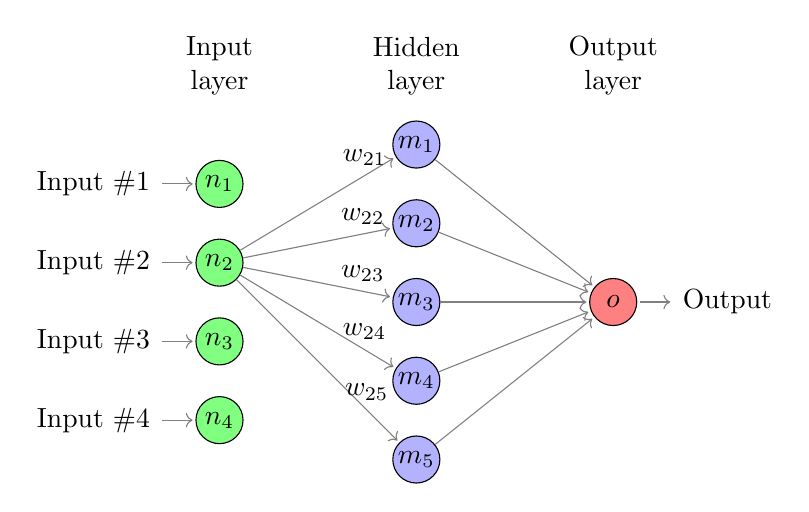
\begin{tikzpicture}[shorten >=1pt,->,draw=black!50, node distance=\layersep]
%https://tex.stackexchange.com/questions/96846/how-to-place-label-in-middle-of-line-above-and-below-with-tikz
    \tikzstyle{every pin edge}=[<-,shorten <=1pt]
    \tikzstyle{neuron}=[circle,fill=black!25,minimum size=17pt,inner sep=0pt, draw=black]
    \tikzstyle{input neuron}=[neuron, fill=green!50];
    \tikzstyle{output neuron}=[neuron, fill=red!50];
    \tikzstyle{hidden neuron}=[neuron, fill=blue!30];
    \tikzstyle{annot} = [text width=4em, text centered]

    % Draw the input layer nodes
    \foreach \name / \y in {1,...,4}
    % This is the same as writing \foreach \name / \y in {1/1,2/2,3/3,4/4}
        \node[input neuron, pin=left:Input \#\y] (I-\name) at (0,-\y) {$n_\y$};

    % Draw the hidden layer nodes
    \foreach \name / \y in {1,...,5}
        \path[yshift=0.5cm]
            node[hidden neuron] (H-\name) at (\layersep,-\y cm) {$m_\y$};

    % Draw the output layer node
    \node[output neuron,pin={[pin edge={->}]right:Output}, right of=H-3] (O) {$o$};

    % Connect every node in the input layer with every node in the
    % hidden layer.
%    \foreach \source in {1,...,4}
%        \foreach \dest in {1,...,5}
%            \draw (I-\source) -- node[below] {$w_ij$} ++ (H-\dest);


%    \foreach \source in {1,...,4}
        \foreach \dest in {1,...,5}
            \draw (I-2) -- node[above, pos=0.8] {$w_{2\dest}$} ++ (H-\dest);

    % Connect every node in the hidden layer with the output layer
    \foreach \source in {1,...,5}
        \path (H-\source) edge (O);

    % Annotate the layers
    \node[annot,above of=H-1, node distance=1cm] (hl) {Hidden layer};
    \node[annot,left of=hl] {Input layer};
    \node[annot,right of=hl] {Output layer};
\end{tikzpicture}
  \end{minipage}
  \vfill
\begin{minipage}[t][0.5\textheight][t]{\textwidth}

\end{minipage}


\end{frame}




\begin{frame}[fragile]{Point Variance of Linear Predictor}

\begin{align*}
\action<+->{ &=&&}
\\
\action<+->{  &=   && }
\end{align*}
\action<+->{The}
\end{frame}



\begin{frame}[fragile]{Correlation}
\begin{itemize}
\item[] \textbf{Serial No.} is basically uncorrelated with anything. \pause
\item[] \textbf{Admit} is highly correlated with \textbf{CGPA}, \textbf{TOEFL Score} and \textbf{GRE Score}\pause
\item[] \textbf{Research} has a lowish correlation with \textbf{Admit}, but also with everything else.  
\end{itemize}
\end{frame}











\begin{frame}[fragile]{Bias, Variance and Parameters}
  \begin{minipage}[t][0.5\textheight][t]{\textwidth}
	\centering
	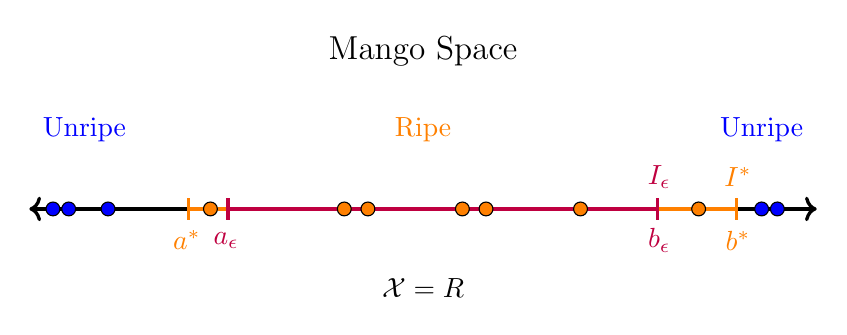
\begin{tikzpicture}
		\draw[<->,very thick] (-5,0) -- (5,0);
		\draw[color = orange, |-|,very thick] (-3,0) -- (4,0);
		\node[color=orange] at (4,.4) {$I^*$};
		\node at (0,2) {\large Mango Space} ;
		\node at (0,-1) {$\mathcal{X} = \mathbb{R}$} ;
		\node [color=blue] at (-4.3,1) {Unripe} ;
		\node [color=blue] at (4.3,1) {Unripe} ;
		\node [color=orange] at (0,1) {Ripe} ;

		\node [color=orange] at (-3,-.4) {$a^*$} ;
		\node [color=orange] at (4,-.4) {$b^*$} ;

		\draw [color=purple, |-|,very thick] (-2.5,0) -- (3,0);
		\node [color=purple] at (3,.4) {$I_\epsilon$} ;
		\node [color=purple] at (-2.5,-.4) {$a_\epsilon$} ;
		\node [color=purple] at (3,-.4) {$b_\epsilon$} ;

%		\draw [color=olive, |-|,very thick] (-3.5,0) -- (2.5,0);
%		\node [color=olive] at (3,.4) {$h_{\mathcal{T}}$} ;



		\node[circle,draw=black, fill=orange, inner sep=0pt,minimum size=5pt] at (2,0) {};
		\node[circle,draw=black, fill=orange, inner sep=0pt,minimum size=5pt] at (-1,0) {};
		\node[circle,draw=black, fill=orange, inner sep=0pt,minimum size=5pt] at (-.7,0) {};
		\node[circle,draw=black, fill=orange, inner sep=0pt,minimum size=5pt] at (.5,0) {};
		\node[circle,draw=black, fill=orange, inner sep=0pt,minimum size=5pt] at (.8,0) {};
		\node[circle,draw=black, fill=orange, inner sep=0pt,minimum size=5pt] at (-2.7,0) {};
		\node[circle,draw=black, fill=orange, inner sep=0pt,minimum size=5pt] at (3.5,0) {};

		\node[circle,draw=black, fill=blue, inner sep=0pt,minimum size=5pt] at (-4.5,0) {};
		\node[circle,draw=black, fill=blue, inner sep=0pt,minimum size=5pt] at (-4,0) {};
		\node[circle,draw=black, fill=blue, inner sep=0pt,minimum size=5pt] at (-4.7,0) {};
		\node[circle,draw=black, fill=blue, inner sep=0pt,minimum size=5pt] at (4.3,0) {};
		\node[circle,draw=black, fill=blue, inner sep=0pt,minimum size=5pt] at (4.5,0) {};
	\end{tikzpicture}
  \end{minipage}
  \vfill
  \begin{minipage}[t][0.5\textheight][t]{\textwidth}
Lets understand this visually.
$$
Err(x_0) = \sigma_\epsilon^2 + [E_\cT[\hat f(x_0)] - f(x_0)]^2 + E_\cT\big[ \hat{f}(x_0) - E_\cT[\hat{f}(x_0)] \big]^2\,.
$$\pause
Consider a data set, 
\end{minipage}
\end{frame}





























